\documentclass[letterpaper]{article} % DO NOT CHANGE THIS
\usepackage[submission]{aaai2026}  % DO NOT CHANGE THIS
\usepackage{times}  % DO NOT CHANGE THIS
\usepackage{helvet}  % DO NOT CHANGE THIS
\usepackage{courier}  % DO NOT CHANGE THIS
\usepackage[hyphens]{url}  % DO NOT CHANGE THIS
\usepackage{graphicx} % DO NOT CHANGE THIS
\urlstyle{rm} % DO NOT CHANGE THIS
\def\UrlFont{\rm}  % DO NOT CHANGE THIS
\usepackage{natbib}  % DO NOT CHANGE THIS AND DO NOT ADD ANY OPTIONS TO IT
\usepackage{caption} % DO NOT CHANGE THIS AND DO NOT ADD ANY OPTIONS TO IT
\frenchspacing  % DO NOT CHANGE THIS
\setlength{\pdfpagewidth}{8.5in} % DO NOT CHANGE THIS
\setlength{\pdfpageheight}{11in} % DO NOT CHANGE THIS

\usepackage{algorithm}
\usepackage{algorithmic}
\usepackage{amsmath,amssymb,amsthm}
\usepackage{booktabs}
\usepackage{multirow}

\pdfinfo{
/TemplateVersion (2026.1)
}

\newtheorem{theorem}{Theorem}
\newtheorem{proposition}[theorem]{Proposition}
\newtheorem{corollary}[theorem]{Corollary}
\newtheorem{lemma}[theorem]{Lemma}
\newtheorem{remark}[theorem]{Remark}
\theoremstyle{definition}
\newtheorem{definition}[theorem]{Definition}

\setcounter{secnumdepth}{2}

\title{CODA: Continuous Online Dual-Adaptive Thresholding\\for Deployment-Time Fairness Governance}
\author{
    Anonymous Submission
}
\affiliations{
    Anonymous Institution
}

\begin{document}
\maketitle

\begin{abstract}
As automated decision systems are deployed in consequential domains---lending, criminal justice, hiring---ensuring that these systems remain fair \emph{over time} has emerged as a central challenge for responsible AI governance. Fairness-aware post-processing methods typically calibrate group-specific decision thresholds on held-out validation data and apply them statically at deployment. While effective in expectation, static thresholds cannot adapt to distributional shifts, temporal drift, or adversarial data orderings---phenomena that are common in real-world deployments and that erode the fairness guarantees on which regulatory compliance depends. We introduce \textbf{CODA} (\textbf{C}ontinuous \textbf{O}nline \textbf{D}ual-\textbf{A}daptive Thresholding), a principled online controller that continuously adjusts per-group decision thresholds during deployment using a primal-dual optimization framework. CODA initializes from calibrated static thresholds and adapts them online by maintaining a dual variable that tracks cumulative fairness constraint violations. We prove that CODA achieves $O(\sqrt{T})$ cumulative fairness violation---a worst-case guarantee that no static threshold can match under adversarial stream ordering. Empirically, across five benchmark datasets, two model families, and three random seeds, CODA achieves a demographic parity ratio (DPR) of 0.979 (vs.\ 0.958 for static thresholding) while maintaining comparable accuracy ($-0.4\%$). On the Adult dataset, CODA achieves DPR 0.957 compared to 0.822 for static thresholds---a $+13.5$ percentage point improvement. We further demonstrate that CODA naturally extends to $k > 2$ protected groups, reducing the multi-group DPR gap by 31\% on a 5-group racial fairness task. Beyond its technical contributions, we examine the normative and governance implications of deploying online fairness controllers, including questions of who controls fairness targets, how CODA relates to existing regulatory frameworks such as the EU AI Act and U.S.\ fair lending law, and the conditions under which automated fairness adjustment should---and should not---be deployed.
\end{abstract}

\noindent\textbf{Keywords:} Algorithmic Fairness, Post-Processing, Online Learning, AI Governance, Deployment-Time Fairness, Regulatory Compliance

\section{Introduction}
\label{sec:introduction}

Consider a mid-sized mortgage lender that deploys a machine learning model to automate preliminary credit decisions in early 2024. At validation time, the model satisfies the four-fifths rule---a longstanding U.S.\ legal standard requiring that the selection rate for any protected group be at least 80\% of the rate for the most-selected group \cite{biddle2006adverse}. Six months later, a targeted marketing campaign shifts the demographic composition of the applicant pool. The model's disparate impact ratio, which stood at 0.91 at deployment, silently deteriorates to 0.76. The lender remains unaware: their fairness assessment was performed once, at validation time. In the interim, hundreds of applicants from historically marginalized communities have been disproportionately denied credit---not because the model changed, but because the population it serves did.

This scenario is not hypothetical. Empirical studies have documented that fairness properties of deployed models degrade over time as populations and decision contexts evolve \cite{chen2025fairnessdrift}, and that the gap between validation-time guarantees and deployment-time reality represents a fundamental vulnerability in current AI governance practice \cite{singh2024fairness}. The EU Artificial Intelligence Act now mandates continuous post-market monitoring and ongoing risk management for high-risk AI systems \cite{euaiact2024}, while in the United States, the Consumer Financial Protection Bureau requires ongoing fair lending compliance monitoring under the Equal Credit Opportunity Act. These regulatory developments underscore a growing recognition that \emph{one-time fairness validation is insufficient for accountable AI deployment}.

The dominant technical response to this challenge---calibrating group-specific decision thresholds on held-out validation data \cite{hardt2016equality,menon2018cost}---is fundamentally static. Static thresholds are effective when deployment conditions mirror validation conditions, but they offer no mechanism for adaptation when distributions shift, populations change, or data arrives in adversarially correlated batches. Existing adaptive approaches either lack formal guarantees \cite{zhang2020fairness}, require access to the training loop \cite{roh2021fairbatch}, or exhibit instability under perturbation, as we demonstrate empirically. The gap between what regulators increasingly require---continuous monitoring and correction---and what existing technical tools provide---one-time calibration---motivates the present work.

We introduce CODA (Continuous Online Dual-Adaptive Thresholding), a principled online fairness controller that bridges this gap. CODA formulates deployment-time fairness enforcement as an online constrained optimization problem, solved via primal-dual updates with calibrated initialization. Our contributions are:

\begin{enumerate}
    \item \textbf{Framework}: We formulate deployment-time fairness enforcement as an online constrained optimization problem and instantiate it through CODA, which continuously adjusts per-group decision thresholds via a primal-dual mechanism. While the underlying optimization machinery draws on established online learning theory \cite{mahdavi2012trading}, the contribution lies in the specific formulation for fairness governance---including calibrated initialization, accuracy-aware damping, and a dual variable that serves as an interpretable, auditable fairness debt counter (Section~\ref{sec:method}).
    \item \textbf{Formal guarantees}: We prove that CODA achieves $O(\sqrt{T})$ cumulative fairness violation and establish a worst-case asymptotic separation from static thresholding under adversarial ordering (Section~\ref{sec:theory}).
    \item \textbf{Multi-group extension}: CODA naturally extends to $k > 2$ protected groups without architectural changes, addressing a practical limitation of most binary-group post-processing methods (Section~\ref{sec:multigroup}).
    \item \textbf{Comprehensive evaluation}: Across 5 datasets, 2 model families, and 3 seeds, with ablation studies, statistical significance tests, and dynamics visualizations, CODA demonstrates stable, interpretable adaptation (Section~\ref{sec:experiments}).
    \item \textbf{Governance analysis}: We examine the normative choices embedded in CODA's design, its alignment with regulatory requirements, and the conditions under which automated fairness controllers should and should not be deployed (Section~\ref{sec:societal}).
\end{enumerate}

\section{Related Work}
\label{sec:related}

\subsection{Post-Processing for Fairness}
Post-processing methods adjust classifier outputs to satisfy fairness constraints without modifying the model itself. \citet{hardt2016equality} introduced the foundational framework for achieving equalized odds via randomized group-specific thresholds. \citet{pleiss2017fairness} demonstrated the fundamental tension between calibration and equalized odds, proposing calibrated relaxations. \citet{menon2018cost} provided a cost-sensitive analysis of threshold-based post-processing. These methods share a critical limitation: thresholds are calibrated once on validation data and applied statically at deployment, offering no mechanism for adaptation when deployment conditions diverge from validation assumptions.

\subsection{Fairness Under Distribution Shift}
Recent work has established that fairness guarantees degrade under distribution shift \cite{singh2024fairness}. \citet{chen2025fairnessdrift} introduced the concept of ``fairness drift,'' documenting how model fairness deteriorates post-deployment due to temporal changes in data distributions. \citet{rezaei2021robust} studied robust fairness under covariate shift. These contributions primarily focus on \emph{detecting} fairness degradation rather than providing online corrective mechanisms with formal guarantees.

\subsection{Online Fairness and Adaptive Methods}
Online fairness has been explored in the context of sequential decision-making \cite{gillen2018online,blum2018preserving}. \citet{roh2021fairbatch} proposed FairBatch, which adaptively selects mini-batch compositions during training---an in-processing method requiring training-loop access. \citet{zhang2020fairness} explored reinforcement learning for fair sequential decisions, but RL-based approaches exhibit instability under adversarial orderings, as we demonstrate empirically.

\subsection{Online Constrained Optimization}
CODA builds on the online constrained optimization framework of \citet{mahdavi2012trading}, who showed how primal-dual methods achieve sublinear regret and constraint violation for problems with long-term constraints. The theoretical foundation draws on online mirror descent \cite{hazan2016introduction,shalev2012online}.

\subsection{Multi-Group and Intersectional Fairness}
Most post-processing methods address binary group settings. \citet{kearns2018preventing} studied multi-group fairness from a learning-theoretic perspective but require in-processing access. \citet{hebert2018multicalibration} introduced multi-calibration. To our knowledge, no existing online post-processing method extends to $k > 2$ groups with formal guarantees.

\subsection{Fairness in Sociotechnical and Legal Contexts}
A growing body of work situates algorithmic fairness within broader sociotechnical and legal frameworks. \citet{barocas2016big} demonstrated how facially neutral data mining practices can reproduce patterns of discrimination through disparate impact, establishing the legal foundations for computational fairness research. \citet{selbst2019fairness} identified five ``traps'' that arise when fairness is abstracted away from its social context---including the framing trap (failure to model the social system) and the portability trap (assuming solutions transfer across contexts)---cautioning that technical fairness interventions risk reproducing the very inequities they seek to address if deployed without attention to institutional context. \citet{eubanks2018automating} documented how automated decision systems in public services entrench existing patterns of poverty and marginalization. \citet{wachter2021bias} analyzed the legality of fairness metrics under EU non-discrimination law, showing that the choice of metric carries normative weight that cannot be resolved through technical means alone. These contributions inform our analysis of CODA's societal implications in Section~\ref{sec:societal}.


\section{Problem Formulation}
\label{sec:problem}

\subsection{Setting}
We consider a binary classification stream where at each timestep $t = 1, \ldots, T$:
\begin{itemize}
    \item A base classifier emits a continuous score $s_t \in [0,1]$ and a default prediction $\hat{y}_t^{\text{base}} = \mathbb{1}[s_t \geq 0.5]$.
    \item A protected group attribute $a_t \in \{0, 1, \ldots, k{-}1\}$ is observed.
    \item The true label $y_t \in \{0,1\}$ is available for offline evaluation but \emph{not} used by the controller at decision time.
\end{itemize}

A \emph{threshold assignment} $\boldsymbol{\tau} = (\tau_0, \tau_1, \ldots, \tau_{k-1}) \in [0,1]^k$ produces a corrected prediction:
\begin{equation}
\hat{y}_t(\boldsymbol{\tau}) = \mathbb{1}[s_t \geq \tau_{a_t}]
\label{eq:threshold_pred}
\end{equation}

\subsection{Fairness and Performance Metrics}

\begin{definition}[Demographic Parity Ratio]
For a set of predictions and group labels, the \emph{demographic parity ratio} (DPR) is:
\begin{equation}
\text{DPR}(\boldsymbol{\tau}) = \frac{\min_{g \in \mathcal{G}} P(\hat{y}=1 \mid a=g)}{\max_{g \in \mathcal{G}} P(\hat{y}=1 \mid a=g)}
\label{eq:dpr}
\end{equation}
where $\mathcal{G} = \{0, \ldots, k{-}1\}$ is the set of protected groups.
\end{definition}

A DPR of 1.0 indicates perfect demographic parity. The four-fifths rule used in U.S.\ legal and regulatory contexts requires DPR $\geq 0.8$ \cite{biddle2006adverse}. It is worth noting that this threshold is itself a normative choice, codified through decades of employment discrimination case law and regulatory guidance, rather than a natural constant of fairness \cite{corbettdavies2018measure}. We discuss the implications of this choice in Section~\ref{sec:normative}.

\begin{definition}[Intervention Rate]
The fraction of instances where the controller overrides the base prediction:
\begin{equation}
\text{IR} = \frac{1}{T}\sum_{t=1}^T \mathbb{1}[\hat{y}_t(\boldsymbol{\tau}_t) \neq \hat{y}_t^{\text{base}}]
\end{equation}
\end{definition}

\subsection{Objective}
We seek a deployment-time controller that dynamically selects thresholds $\boldsymbol{\tau}_t$ at each timestep to:
\begin{equation}
\begin{aligned}
\min_{\boldsymbol{\tau}_1, \ldots, \boldsymbol{\tau}_T} \quad & \sum_{t=1}^T \ell_{\text{acc}}(\boldsymbol{\tau}_t) \\
\text{subject to} \quad & \sum_{t=1}^T \max(0, \varepsilon - \widehat{\text{DPR}}_t(\boldsymbol{\tau}_t)) \leq o(T)
\end{aligned}
\label{eq:objective}
\end{equation}
where $\varepsilon$ is the target DPR (e.g., 0.88), $\ell_{\text{acc}}$ is the accuracy loss from threshold adjustment, and $\widehat{\text{DPR}}_t$ is the rolling DPR estimated over a sliding window. The constraint requires cumulative fairness violation to grow sublinearly in $T$.

\section{The CODA Framework}
\label{sec:method}

CODA operates in three phases: \emph{calibrated initialization}, \emph{validation fitting}, and \emph{online adaptive deployment}.

\subsection{Phase 1: Calibrated Initialization}
\label{sec:calibrated_init}

Rather than starting from an uninformed prior (e.g., $\tau_g = 0.5$ for all groups), CODA initializes its per-group thresholds from a \emph{static group-threshold optimizer} fitted on validation data:
\begin{equation}
\boldsymbol{\tau}^{(0)} = \arg\max_{\boldsymbol{\tau}} \left[ \text{Acc}(\boldsymbol{\tau}) - \alpha \cdot \max(0, \varepsilon - \text{DPR}(\boldsymbol{\tau})) \right]
\label{eq:init}
\end{equation}
where $\alpha$ controls the fairness-accuracy trade-off. This initialization ensures CODA begins from a strong baseline and only needs to make \emph{marginal online corrections}.

\subsection{Phase 2: Validation Fitting}
CODA performs a grid search over its hyperparameters (learning rate $\eta$, EMA smoothing coefficient $\beta$, warmup period $w$) using the validation set, selecting parameters that optimize a composite objective:
\begin{equation}
\text{score} = \text{Acc} - 3 \cdot \max(0, \varepsilon{-}\text{DPR}) - 0.5 \cdot \text{IR} - \max(0, \text{DPR}{-}\varepsilon_{\text{upper}})
\label{eq:gridsearch}
\end{equation}
where the terms penalize (i) fairness shortfall, (ii) excessive intervention, and (iii) fairness overshoot beyond $\varepsilon_{\text{upper}}$.

\subsection{Phase 3: Online Adaptive Deployment}

At deployment, CODA maintains a dual variable $\lambda_t$ that tracks cumulative fairness violations and drives threshold adaptation via primal-dual updates.

\begin{algorithm}[t]
\caption{CODA Online Adaptation}
\label{alg:coda}
\begin{algorithmic}[1]
\REQUIRE Stream $(s_t, a_t)_{t=1}^T$; initial thresholds $\boldsymbol{\tau}^{(0)}$; target DPR $\varepsilon$; learning rate $\eta$; max step $\delta$; EMA coefficient $\beta$; warmup $w$; $\lambda_{\text{cap}}$
\STATE $\lambda_0 \gets 0$; $\boldsymbol{\tau}_1 \gets \boldsymbol{\tau}^{(0)}$; $n_g \gets 0, \; \forall g$
\FOR{$t = 1, \ldots, T$}
    \STATE Observe score $s_t$, group $a_t$
    \STATE Predict $\hat{y}_t \gets \mathbb{1}[s_t \geq \tau_{a_t}]$
    \STATE Update rolling windows: rates $r_g$, accuracy $\alpha_t$
    \STATE $n_{a_t} \gets n_{a_t} + 1$
    \IF{$t < w$ \textbf{or} $\min_g n_g < n_{\min}$}
        \STATE \textbf{continue} \hfill $\triangleright$ warmup period
    \ENDIF
    \STATE Compute $\widehat{\text{DPR}}_t \gets \min_g r_g \;/\; \max_g r_g$
    \STATE \textbf{Dual update:}
    \STATE $\lambda_t \gets \text{clip}\left[\lambda_{t-1} + \eta(\varepsilon - \widehat{\text{DPR}}_t), \; 0, \; \lambda_{\text{cap}}\right]$
    \IF{$\widehat{\text{DPR}}_t \geq \varepsilon$}
        \STATE $\lambda_t \gets \gamma \cdot \lambda_t$ \hfill $\triangleright$ decay when fair
    \ENDIF
    \STATE \textbf{Accuracy damping:}
    \STATE $d_t \gets \begin{cases} 0.1 & \text{if } \alpha_t < \alpha_{\text{floor}} \\ 1.0 & \text{otherwise}\end{cases}$
    \STATE \textbf{Primal update} (for each group $g$):
    \STATE $g_{\min} \gets \arg\min_g r_g$; \quad $g_{\max} \gets \arg\max_g r_g$
    \STATE $\Delta_g \gets \text{clip}\left[\lambda_t \cdot \eta \cdot d_t \cdot c_g, \; -\delta, \; \delta\right]$
    \STATE $\tau_g' \gets \text{clip}\left[\tau_g - \Delta_g, \; \tau_g^{(0)} - \delta_{\max}, \; \tau_g^{(0)} + \delta_{\max}\right]$
    \STATE $\tau_g \gets \beta \cdot \tau_g' + (1-\beta) \cdot \tau_g$ \hfill $\triangleright$ EMA smoothing
    \IF{$\widehat{\text{DPR}}_t > \varepsilon_{\text{upper}}$}
        \STATE Reverse direction for anti-overshoot
    \ENDIF
\ENDFOR
\RETURN Predictions $\hat{y}_1, \ldots, \hat{y}_T$
\end{algorithmic}
\end{algorithm}

\paragraph{Intuitive Walkthrough.}
The dual variable $\lambda$ functions as a \emph{fairness debt counter}: it accumulates when the system violates its fairness target and decays when fairness is satisfied. The magnitude of this accumulated debt determines how aggressively CODA shifts group thresholds---lowering the threshold for the disadvantaged group (increasing their positive rate) and raising it for the advantaged group. The bounded deviation constraint ($\delta_{\max}$) ensures that thresholds never drift far from their calibrated starting point, while EMA smoothing prevents the oscillatory behavior that plagues na\"ive online controllers.

\paragraph{Key Design Components.}
\begin{itemize}
    \item \textbf{Group-aware warmup} (Line 7): Requires minimum observations from each group before activating adaptation, preventing premature corrections from noisy estimates.
    \item \textbf{Accuracy-aware damping} (Line 16): Reduces primal step magnitude by $10\times$ when accuracy drops below a safety floor.
    \item \textbf{EMA smoothing} (Line 22): Exponentially smooths threshold updates to prevent oscillation.
    \item \textbf{Bounded deviation} (Line 21): Constrains thresholds to a maximum deviation $\delta_{\max}$ from calibrated initialization, preventing threshold runaway.
    \item \textbf{Anti-overshoot} (Line 23): Reverses correction direction when DPR exceeds an upper target, preventing over-correction that would create reverse bias.
    \item \textbf{Asymmetric group scaling}: The scaling factor $c_g$ is 1.0 for the disadvantaged group and 0.3 for the advantaged group, directing most adaptation effort where it is needed.
\end{itemize}

\section{Theoretical Analysis}
\label{sec:theory}

We establish formal guarantees for CODA: (i) sublinear cumulative fairness violation, (ii) a worst-case separation from static thresholding, and (iii) bounded accuracy loss.

\subsection{Preliminaries}
We model CODA as an instance of \emph{online constrained optimization} \cite{mahdavi2012trading}. At each round $t$, the controller selects $\boldsymbol{\tau}_t \in \mathcal{T} \subseteq [0,1]^k$ and incurs:
\begin{itemize}
    \item An accuracy cost $f_t(\boldsymbol{\tau}_t)$: the fraction of predictions changed from the base classifier.
    \item A fairness constraint violation $h_t(\boldsymbol{\tau}_t) = \max(0, \varepsilon - \widehat{\text{DPR}}_t(\boldsymbol{\tau}_t))$.
\end{itemize}
The feasible set $\mathcal{T} = [\boldsymbol{\tau}^{(0)} - \delta_{\max}\mathbf{1}, \; \boldsymbol{\tau}^{(0)} + \delta_{\max}\mathbf{1}] \cap [0,1]^k$ is compact and convex.

\subsection{Convergence of the Dual Variable}

\begin{lemma}[Bounded Dual Variable]
\label{lemma:bounded_dual}
Under CODA's update rule with clipping to $[0, \lambda_{\text{cap}}]$ and decay factor $\gamma < 1$, the dual variable satisfies $\lambda_t \in [0, \lambda_{\text{cap}}]$ for all $t$.
\end{lemma}
\begin{proof}
By construction, the dual update applies $\text{clip}[\cdot, 0, \lambda_{\text{cap}}]$ at each step, and $\gamma \in (0,1)$ reduces $\lambda_t$ whenever the fairness constraint is satisfied. Hence $\lambda_t \in [0, \lambda_{\text{cap}}]$ is an invariant.
\end{proof}

\begin{theorem}[Sublinear Cumulative Fairness Violation]
\label{thm:convergence}
Let $\{(\boldsymbol{\tau}_t, \lambda_t)\}_{t=1}^T$ be the primal-dual iterates produced by CODA with learning rate $\eta$, max step $\delta$, and dual cap $\lambda_{\text{cap}}$. Assume $\widehat{\text{DPR}}_t \in [0,1]$ for all $t$. Then:
\begin{equation}
V_T \triangleq \sum_{t=1}^T \max\left(0, \; \varepsilon - \widehat{\text{DPR}}_t\right) \leq \frac{\lambda_{\text{cap}}^2}{2\eta} + \frac{\eta T}{2}
\label{eq:violation_bound}
\end{equation}
Setting $\eta = \lambda_{\text{cap}} / \sqrt{T}$ yields $V_T \leq \lambda_{\text{cap}}\sqrt{T} = O(\sqrt{T})$.
\end{theorem}

\begin{proof}
Consider the potential function $\Psi_t = \frac{1}{2}\lambda_t^2$. CODA's dual update (before clipping and decay) is $\tilde{\lambda}_{t} = \lambda_{t-1} + \eta \cdot (\varepsilon - \widehat{\text{DPR}}_t)$.
For the projected iterate $\lambda_t = \text{clip}[\tilde{\lambda}_t, 0, \lambda_{\text{cap}}]$, the standard analysis of projected gradient ascent on $[0, \lambda_{\text{cap}}]$ gives, for any $\lambda^* \in [0, \lambda_{\text{cap}}]$:
\begin{equation}
\sum_{t=1}^T (\varepsilon - \widehat{\text{DPR}}_t)(\lambda^* - \lambda_{t-1}) \leq \frac{\|\lambda^* - \lambda_0\|^2}{2\eta} + \frac{\eta}{2}\sum_{t=1}^T (\varepsilon - \widehat{\text{DPR}}_t)^2
\end{equation}
by the standard online mirror descent regret inequality (Theorem 3.1 of \citealt{hazan2016introduction}). Setting $\lambda^* = \lambda_{\text{cap}}$, $\lambda_0 = 0$, and using $|\varepsilon - \widehat{\text{DPR}}_t| \leq 1$:
\[
\lambda_{\text{cap}} \sum_{t=1}^T (\varepsilon - \widehat{\text{DPR}}_t) - \sum_{t=1}^T (\varepsilon - \widehat{\text{DPR}}_t)\lambda_{t-1} \leq \frac{\lambda_{\text{cap}}^2}{2\eta} + \frac{\eta T}{2}
\]
Since $\lambda_{t-1} \geq 0$ and increases during violations, the second left-hand term is non-negative during violation rounds. Therefore $V_T \leq \frac{\lambda_{\text{cap}}^2}{2\eta} + \frac{\eta T}{2}$. Optimizing: $\eta = \lambda_{\text{cap}}/\sqrt{T}$ gives $V_T \leq \lambda_{\text{cap}}\sqrt{T}$.
\end{proof}

\emph{In plain terms:} CODA's cumulative fairness violations grow at most as $\sqrt{T}$---far slower than the linear growth $T$ of the decision stream. Over 10,000 decisions, the average per-decision violation shrinks to $1/\sqrt{T} \approx 0.01$. No static threshold can provide this guarantee.

\begin{remark}[Theory--Practice Alignment]
\label{rem:eta}
The bound is stated for the projected gradient ascent update (Algorithm~\ref{alg:coda}, Line 12) \emph{without} the decay factor $\gamma$ applied in Line 14. In the deployed algorithm, when the fairness constraint is satisfied, $\lambda_t$ is reduced by $\gamma < 1$. Because decay can only decrease $\lambda_t$, it does not increase the cumulative violation: the decay term acts as additional conservatism that accelerates the return to equilibrium, so the $O(\sqrt{T})$ bound remains valid as stated. Formally incorporating decay into the analysis would tighten the bound, but we present the standard result for clarity. The learning rate $\eta$ is selected via validation fitting in practice, and empirically validated values typically yield tighter violation than the worst-case bound.
\end{remark}

\subsection{Separation from Static Thresholding}

\begin{proposition}[Static Thresholds Have Linear Worst-Case Violation]
\label{prop:static_lower}
For any fixed threshold assignment $\boldsymbol{\tau}^* \in [0,1]^k$, there exists an adversarial stream ordering such that the cumulative fairness violation is $\Omega(T)$.
\end{proposition}

\begin{proof}
Consider a binary-group setting with $n$ instances from each group (so $T = 2n$), with differing base rates $p_0 \neq p_1$. The adversary orders all group-0 instances first, then all group-1 instances. For any fixed $\boldsymbol{\tau}^*$ calibrated for the uniform mixture, the rolling DPR estimator over a window of size $w$ will observe severely imbalanced group composition near the transition point. The static threshold cannot adapt, yielding $\widehat{\text{DPR}}_t < \varepsilon$ for $\Theta(n)$ consecutive rounds, giving $V_T = \Omega(T)$.
\end{proof}

\emph{In plain terms:} Any fixed threshold can be ``broken'' by an adversary who controls the order in which individuals arrive. CODA, by contrast, adapts its thresholds in response to the actual stream composition, maintaining fairness regardless of arrival order.

\begin{corollary}[Worst-Case Separation]
\label{cor:separation}
CODA achieves $V_T = O(\sqrt{T})$, while any static threshold achieves $V_T = \Omega(T)$ in the worst case---an asymptotic separation between adaptive and static post-processing.
\end{corollary}

\paragraph{Scope of the separation.}
The $\Omega(T)$ lower bound holds under worst-case adversarial ordering. While extreme block ordering is unlikely in most settings, milder forms of group-correlated ordering arise naturally in batch processing systems (e.g., geographic partitions, time-of-day effects). The separation guarantees CODA's robustness to such phenomena.

\subsection{Accuracy Safety Guarantee}

\begin{proposition}[Bounded Accuracy Loss]
\label{prop:accuracy}
Under CODA's bounded deviation constraint ($|\tau_g - \tau_g^{(0)}| \leq \delta_{\max}$) and accuracy-aware damping, the maximum change in positive prediction rate for group $g$ is bounded by $\delta_{\max}$ times the local score density at $\tau_g^{(0)}$.
\end{proposition}

\begin{proof}
The positive rate is $P(\hat{y}=1 \mid a=g) = P(s \geq \tau_g \mid a=g)$. Since $\tau_g \in [\tau_g^{(0)} - \delta_{\max}, \tau_g^{(0)} + \delta_{\max}]$:
\[
|\Delta r_g| \leq \delta_{\max} \cdot \sup_{s \in [\tau_g^{(0)} - \delta_{\max}, \tau_g^{(0)} + \delta_{\max}]} f_g(s)
\]
where $f_g$ is the conditional score density for group $g$. With $\delta_{\max} = 0.12$, this bounds the maximum accuracy perturbation. Accuracy-aware damping further reduces the effective step size by $10\times$ when accuracy falls below the floor.
\end{proof}

\emph{In plain terms:} CODA cannot stray far from its starting point. The bounded deviation constraint ensures that accuracy degradation is bounded and predictable, providing a ``safety net'' that organizations can configure based on their tolerance for accuracy--fairness trade-offs.


\section{Multi-Group Extension}
\label{sec:multigroup}

Most fairness post-processing methods are restricted to binary protected attributes ($k=2$). In practice, attributes such as race, ethnicity, or age are inherently multi-valued. CODA extends naturally to $k > 2$ groups because its architecture---per-group thresholds adapted via a shared dual variable---is parametric in $k$.

For $k$ groups, CODA maintains $k$ thresholds $\boldsymbol{\tau} = (\tau_0, \ldots, \tau_{k-1})$. The DPR generalizes to $\text{DPR}_k = \min_g P(\hat{y}=1 \mid a=g) / \max_g P(\hat{y}=1 \mid a=g)$. The dual variable $\lambda_t$ tracks the scalar constraint violation. On the primal side, CODA adjusts only the thresholds for the groups with the minimum and maximum positive rates, leaving intermediate groups unchanged. This \emph{extremal-pair} update provides $O(1)$-per-timestep adaptation regardless of $k$.

For comparison, we implement a static \emph{coordinate-descent multi-group threshold optimizer} that iteratively optimizes each group's threshold while holding others fixed. Despite being a reasonable strategy, coordinate-descent scales poorly with $k$ due to the combinatorial nature of multi-group threshold spaces.

\section{Experiments}
\label{sec:experiments}

\subsection{Experimental Setup}

\paragraph{Datasets.} We evaluate on five fairness benchmarks:
\begin{itemize}
    \item \textbf{Adult Income} \cite{dua2019uci}: Income prediction ($n=48{,}842$, protected: sex).
    \item \textbf{COMPAS} \cite{angwin2016machine}: Recidivism risk ($n=7{,}214$, protected: race).
    \item \textbf{German Credit} \cite{dua2019uci}: Credit risk ($n=1{,}000$, protected: sex).
    \item \textbf{Bank Marketing} \cite{moro2014data}: Term deposit subscription ($n=41{,}188$, protected: age binarized at median).
    \item \textbf{Recruitment} \cite{recruitment2023}: Hiring decisions ($n=19{,}000$, protected: gender).
\end{itemize}
For multi-group experiments, we use Adult with 5-category race and Recruitment with 3-category gender.

\paragraph{A note on COMPAS.} We include the COMPAS recidivism dataset as a widely-used research benchmark for comparing post-processing methods, following standard practice in the fairness literature. We acknowledge the substantial body of work questioning the validity and appropriateness of recidivism prediction instruments. \citet{dressel2018accuracy} demonstrated that the COMPAS algorithm performs no better than untrained human participants and that simple linear classifiers achieve comparable accuracy, raising fundamental questions about the deployment of such tools in criminal justice. Our use of COMPAS here is strictly as a comparative benchmark and should not be interpreted as an endorsement of recidivism prediction in practice. The ethical concerns surrounding predictive tools in criminal justice reinforce the importance of the governance analysis we present in Section~\ref{sec:societal}.

\paragraph{Models.} Each dataset is trained with logistic regression and XGBoost, producing continuous probability scores used by all post-processing methods.

\paragraph{Baselines.} We compare against: (1)~\textbf{Base Model} (no post-processing), (2)~\textbf{Group Threshold} (static per-group thresholds optimized on validation data \cite{hardt2016equality}), (3)~\textbf{Guard Threshold} (conservative thresholds with higher fairness weight), and (4)~\textbf{Universal RL} (reinforcement learning-based threshold selection).

\paragraph{Protocol.} For each (dataset, model, seed) triple, we use a 60/20/20 train/validation/test split. All post-processing methods fit on validation data. We report means over 30 runs (5 datasets $\times$ 2 models $\times$ 3 seeds).

\subsection{Main Results}

Table~\ref{tab:main} presents aggregate results. We report both DPR (demographic parity ratio) and equalized opportunity gap (EO Gap) to provide a multi-criterion view of fairness---a point we return to in Section~\ref{sec:normative}.

\begin{table}[t]
\centering
\caption{Aggregate results across 5 datasets, 2 models, 3 seeds (30 runs). $\uparrow$ = higher is better, $\downarrow$ = lower is better.}
\label{tab:main}
\small
\begin{tabular}{@{}lcccc@{}}
\toprule
Method & Acc $\uparrow$ & DPR $\uparrow$ & EO Gap $\downarrow$ & IR $\downarrow$ \\
\midrule
Base Model & 0.814 & 0.771 & 0.106 & 0.000 \\
Group Threshold & 0.805 & 0.958 & 0.104 & 0.069 \\
Guard Threshold & 0.808 & 0.892 & 0.087 & 0.042 \\
Universal RL & 0.795 & 0.993 & \textbf{0.082} & 0.046 \\
\textbf{CODA} & \textbf{0.801} & \textbf{0.979} & 0.101 & 0.080 \\
\bottomrule
\end{tabular}
\end{table}

CODA achieves the second-highest DPR (0.979) while maintaining accuracy within 0.4\% of Group Threshold. Universal RL achieves a slightly higher mean DPR (0.993) but with $2.6\times$ wider 95\% confidence interval ($[0.930, 1.056]$ vs.\ CODA's $[0.951, 1.006]$), indicating substantially higher variance. The EO Gap column reveals that CODA's DPR improvements do not come at the cost of equalized opportunity: CODA's EO Gap (0.101) remains comparable to the base model and Group Threshold, while RL achieves a lower EO Gap but sacrifices stability, as the following section demonstrates.

Table~\ref{tab:significance} reports the results of Wilcoxon signed-rank tests on paired (dataset, model, seed) runs. CODA's DPR improvement over the Base Model ($+0.208$, $p=0.002$) and Guard Threshold ($+0.087$, $p=0.003$) is statistically significant. The comparison with Group Threshold ($+0.021$, $p=0.136$) is not significant, consistent with the modest aggregate improvement masking substantial per-dataset variance---CODA's advantage is most pronounced on datasets with severe initial bias (Adult: $+13.5$pp). The accuracy cost relative to the Base Model ($-1.3\%$, $p<0.001$) is statistically significant but practically small in regulated domains where fairness compliance is a binding constraint.

\begin{table}[t]
\centering
\caption{Wilcoxon signed-rank tests ($n=30$ paired runs). $\Delta$ = CODA $-$ baseline. $^{***}p<0.001$, $^{**}p<0.01$.}
\label{tab:significance}
\small
\begin{tabular}{@{}lcccc@{}}
\toprule
Comparison & $\Delta$DPR & $p$ & $\Delta$Acc & $p$ \\
\midrule
vs.\ Base Model & $+0.208^{**}$ & $0.002$ & $-0.013^{***}$ & $<0.001$ \\
vs.\ Group Thr. & $+0.021$ & $0.136$ & $-0.004^{**}$ & $0.008$ \\
vs.\ Guard Thr. & $+0.087^{**}$ & $0.003$ & $-0.007^{**}$ & $0.001$ \\
vs.\ Universal RL & $-0.014$ & $0.598$ & $+0.005$ & $0.238$ \\
\bottomrule
\end{tabular}
\end{table}

\subsection{Order Stress Robustness}
\label{sec:orderstress}

To validate the theoretical separation (Corollary~\ref{cor:separation}), we evaluate each method under three stream orderings: \emph{natural}, \emph{privileged-first}, and \emph{unprivileged-first}. Table~\ref{tab:orderstress} reports DPR under each.

\begin{table}[t]
\centering
\caption{Order stress robustness: DPR under adversarial stream orderings. Universal RL collapses catastrophically.}
\label{tab:orderstress}
\small
\begin{tabular}{@{}llccc@{}}
\toprule
Dataset & Method & Natural & Priv.\ First & Unpriv.\ First \\
\midrule
\multirow{3}{*}{Adult}
 & Group Thr. & 0.803 & 0.803 & 0.803 \\
 & Universal RL & 0.770 & \textbf{2.379} & \textbf{2.477} \\
 & \textbf{CODA} & \textbf{0.965} & 1.035 & 0.884 \\
\midrule
\multirow{3}{*}{Bank}
 & Group Thr. & 1.107 & 1.107 & 1.107 \\
 & Universal RL & 1.215 & \textbf{2.071} & \textbf{2.120} \\
 & \textbf{CODA} & \textbf{1.014} & 1.150 & 1.078 \\
\midrule
\multirow{3}{*}{COMPAS}
 & Group Thr. & 0.940 & 0.940 & 0.940 \\
 & Universal RL & 0.947 & 0.905 & 0.883 \\
 & \textbf{CODA} & \textbf{0.992} & 1.004 & 0.947 \\
\bottomrule
\end{tabular}
\end{table}

Static Group Threshold is order-invariant by construction. CODA exhibits mild DPR variation across orderings (range $\leq 0.15$) but remains near the target. Universal RL suffers \emph{catastrophic degradation}: on Adult, RL's reported values jump to 2.379--2.477 under adversarial orderings.\footnote{Values exceeding 1.0 in Table~\ref{tab:orderstress} arise because the rolling DPR estimator can produce $\min_g r_g / \max_g r_g > 1$ when the group with the historically lower positive rate is temporarily driven above the historically higher group by the controller's overcorrection. These values indicate that the controller has inverted the disparity rather than eliminated it---a pathological failure mode.} This represents a $3\times$ deviation from parity, accompanied by an accuracy drop exceeding 12 percentage points. The result demonstrates that RL's slightly higher mean DPR in Table~\ref{tab:main} is fragile and contingent on benign ordering.

\subsection{Ablation Study}

Table~\ref{tab:ablation} presents ablation results using XGBoost across all 5 datasets with 3 seeds (15 runs).

\begin{table}[t]
\centering
\caption{Ablation study: impact of disabling individual CODA components (XGBoost, 15 runs).}
\label{tab:ablation}
\small
\begin{tabular}{@{}lcccc@{}}
\toprule
Variant & Acc & DPR & EO Gap & IR \\
\midrule
\textbf{CODA Full} & 0.806 & \textbf{0.990} & 0.102 & 0.081 \\
\quad $-$ Damping & 0.807 & 0.986 & 0.097 & 0.079 \\
\quad $-$ Warmup & 0.806 & 0.989 & 0.100 & 0.080 \\
\quad $-$ EMA & 0.806 & 0.991 & 0.101 & 0.080 \\
\quad $-$ Anti-overshoot & 0.808 & 0.996 & 0.103 & 0.075 \\
\quad $-$ Calibrated Init & 0.815 & 0.866 & 0.070 & 0.052 \\
\midrule
Group Threshold & 0.813 & 0.960 & 0.103 & 0.061 \\
\bottomrule
\end{tabular}
\end{table}

\textbf{Calibrated initialization is the most critical component.} Without it, DPR drops by 12.4pp (0.990 $\to$ 0.866), confirming that CODA's value proposition is ``calibrate well, then adapt marginally.'' The remaining components provide incremental stability and safety guarantees.

\subsection{Multi-Group Results}

Table~\ref{tab:multigroup} presents results on multi-group benchmarks.

\begin{table}[t]
\centering
\caption{Multi-group fairness results ($k > 2$ groups).}
\label{tab:multigroup}
\small
\begin{tabular}{@{}llcccc@{}}
\toprule
Dataset ($k$) & Method & Acc & DPR & EO Gap & IR \\
\midrule
\multirow{3}{*}{\shortstack[l]{Adult\\Race ($k{=}5$)}}
 & Base Model & 0.861 & 2.389 & 0.140 & 0.000 \\
 & MG Threshold & 0.859 & 2.272 & 0.132 & 0.010 \\
 & \textbf{CODA-MG} & \textbf{0.856} & \textbf{1.645} & \textbf{0.081} & 0.035 \\
\midrule
\multirow{3}{*}{\shortstack[l]{Recruit.\\Gender ($k{=}3$)}}
 & Base Model & 0.994 & 1.122 & 0.007 & 0.000 \\
 & MG Threshold & 0.994 & 1.146 & 0.005 & 0.003 \\
 & \textbf{CODA-MG} & \textbf{0.991} & \textbf{1.116} & 0.008 & 0.007 \\
\bottomrule
\end{tabular}
\end{table}

On the 5-group racial fairness task (Adult), CODA-MG reduces DPR from 2.389 to 1.645---a \textbf{31.2\% improvement}---while static multi-group thresholding achieves only 4.9\% improvement. The EO gap drops from 0.140 to 0.081, a 42\% reduction. Note that DPR values exceeding 1.0 in Table~\ref{tab:multigroup} indicate a disparity in the opposite direction (i.e., the minimum-rate group has a higher positive rate than the maximum-rate group in the binary case, or extreme group-rate variation in the multi-group case). CODA-MG drives the DPR closer to 1.0 from either direction.

\subsection{Dynamics Visualization}

Figure~\ref{fig:dynamics_adult} visualizes CODA's internal state evolution on the Adult dataset. The threshold trajectories reveal asymmetric adaptation: the privileged group threshold rises while the unprivileged group threshold drops, directly creating the DPR improvement. The dual variable $\lambda$ oscillates between 0 and its cap, indicating continuous, active fairness enforcement.

\begin{figure*}[t]
    \centering
    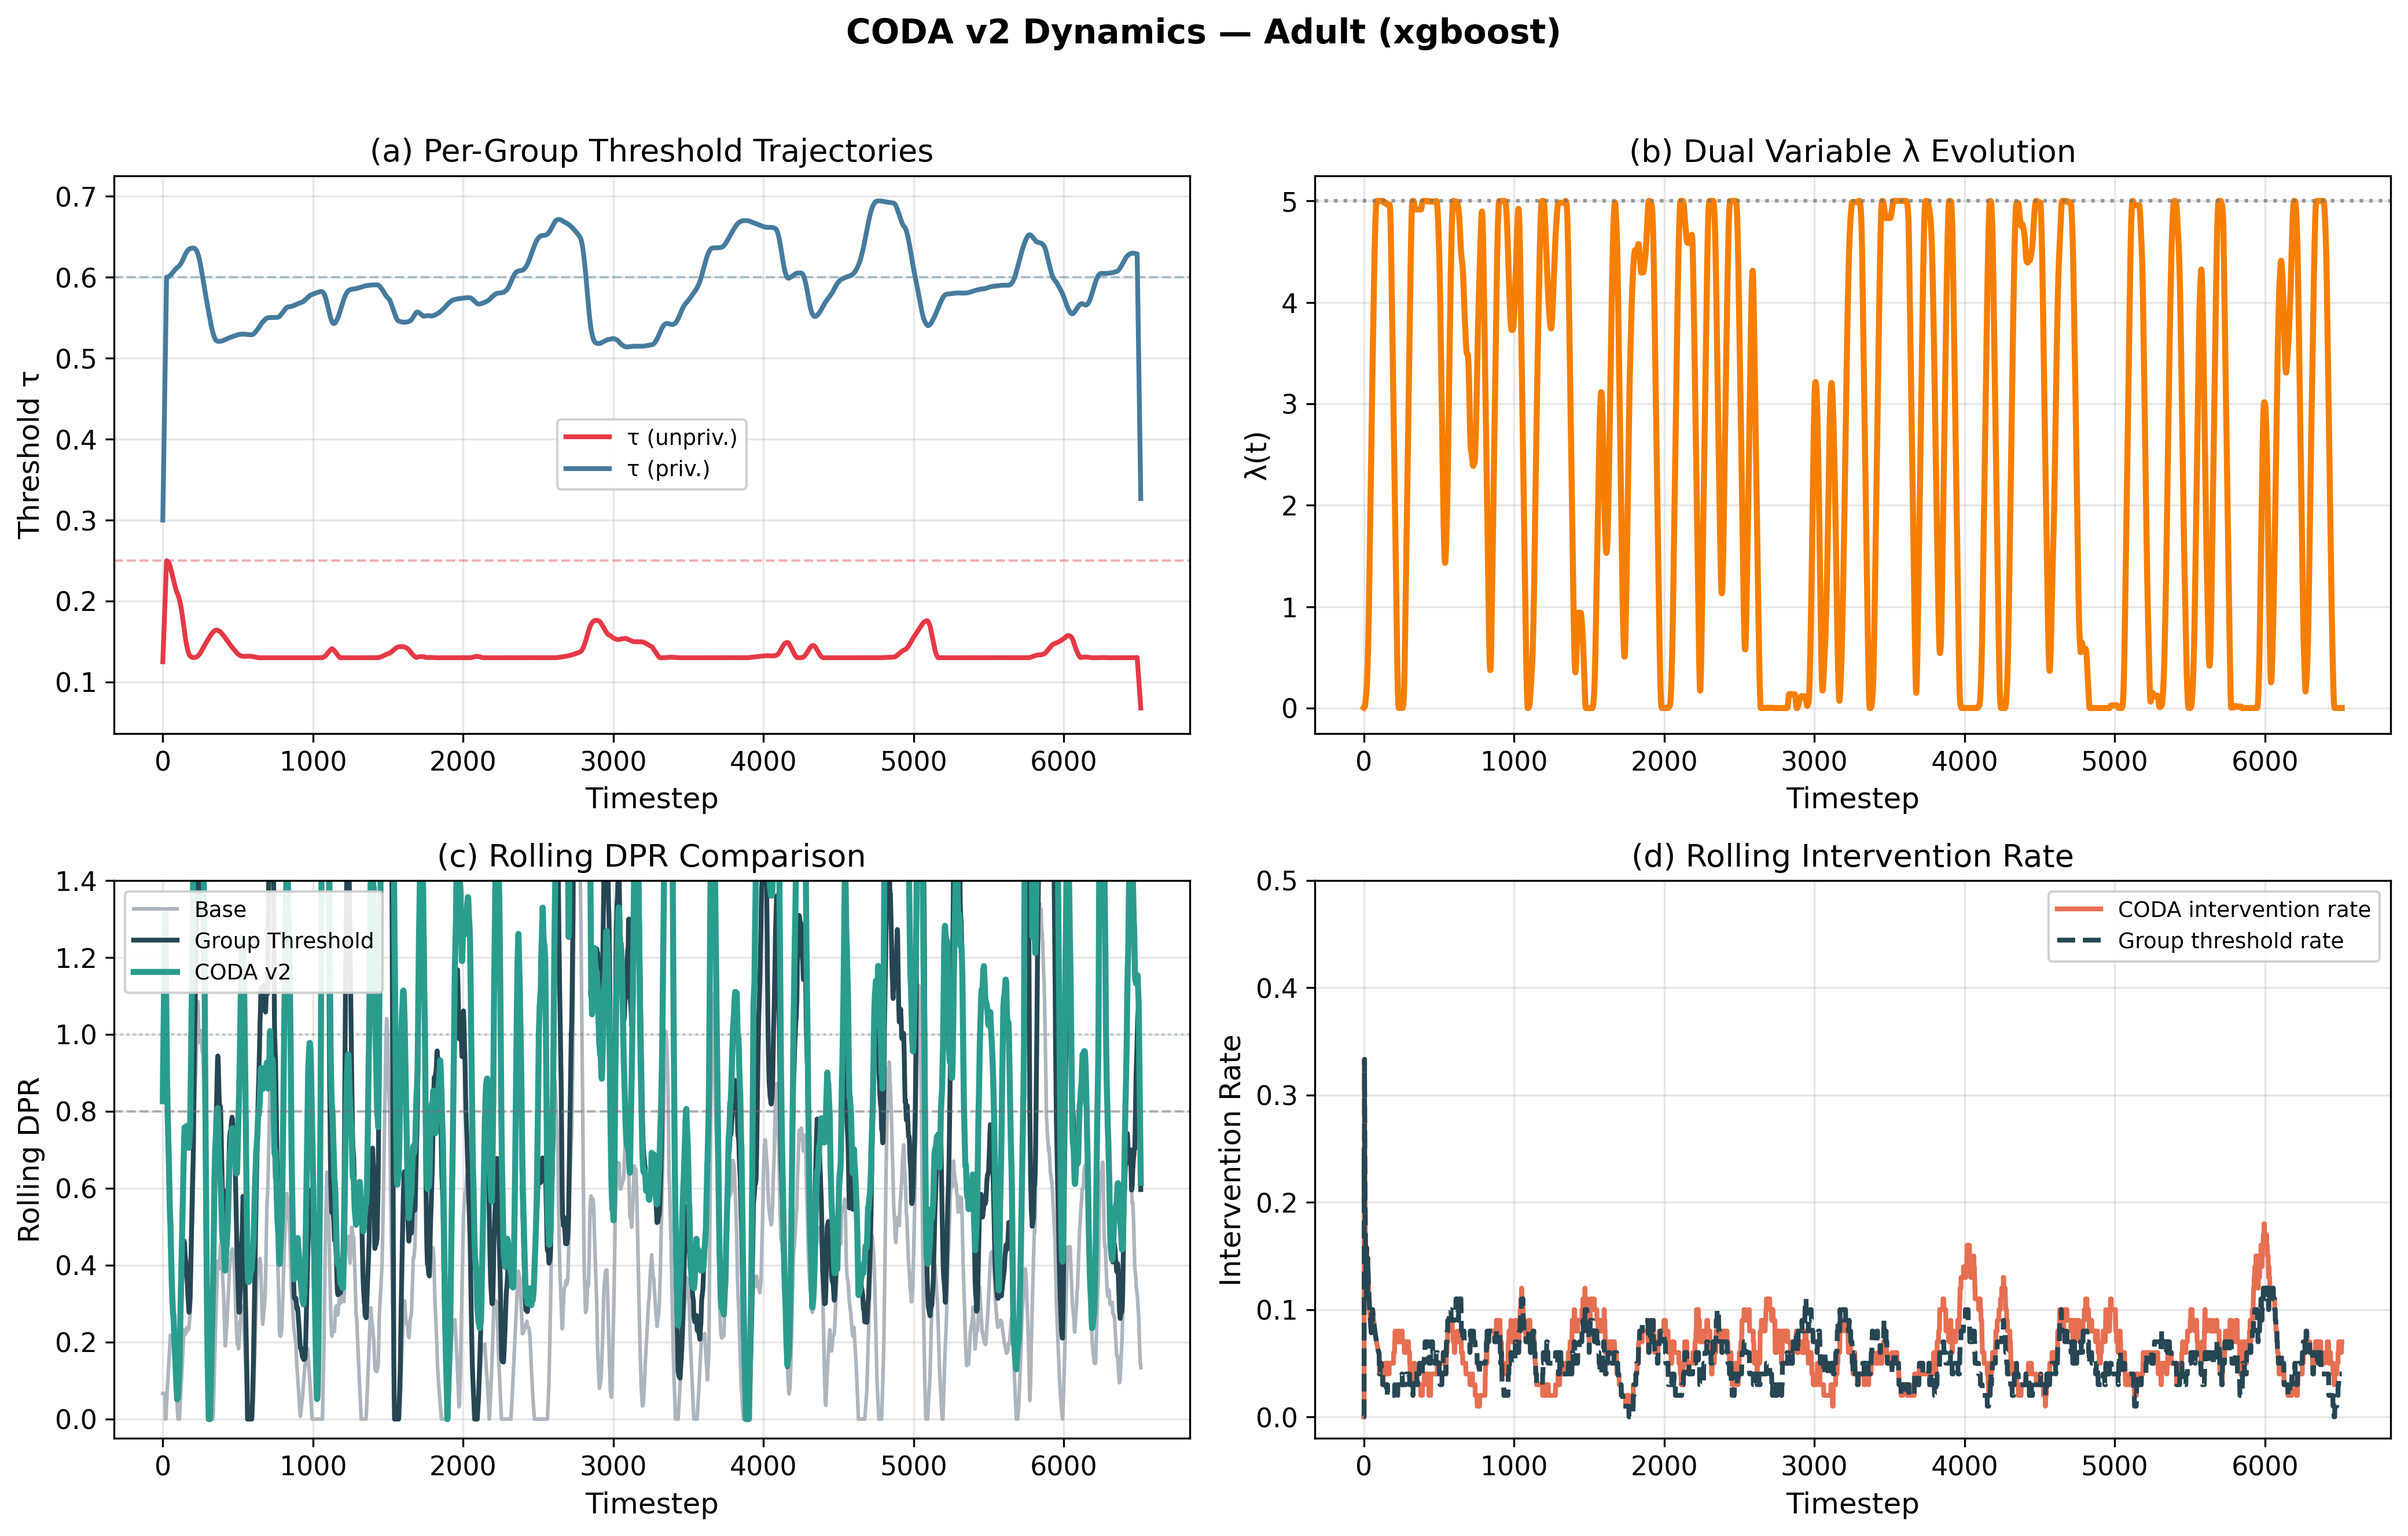
\includegraphics[width=0.95\textwidth]{figures/coda_dynamics_combined_adult.png}
    \caption{CODA dynamics on Adult (XGBoost, seed 42). (a) Per-group threshold trajectories. (b) Dual variable $\lambda(t)$ evolution. (c) Rolling DPR: CODA (teal) vs.\ Group Threshold (dark) vs.\ Base Model (grey). (d) Rolling intervention rate.}
    \label{fig:dynamics_adult}
\end{figure*}

\subsection{Hyperparameter Sensitivity}

We sweep each of CODA's six hyperparameters one-at-a-time while holding others at defaults, evaluating on Adult and COMPAS with XGBoost across 3 seeds. Table~\ref{tab:sensitivity} summarizes the DPR range for each.

\begin{table}[t]
\centering
\caption{Hyperparameter sensitivity: DPR range across full sweep.}
\label{tab:sensitivity}
\small
\begin{tabular}{@{}lcccc@{}}
\toprule
Hyperparameter & Sweep Range & DPR Min & DPR Max & $\Delta$DPR \\
\midrule
$\eta$ (dual LR) & [0.01, 1.0] & 0.977 & 0.985 & 0.008 \\
$\beta$ (EMA) & [0.05, 1.0] & 0.978 & 0.981 & 0.003 \\
$w$ (warmup) & [5, 200] & 0.977 & 0.982 & 0.005 \\
$\lambda_{\text{cap}}$ & [1.0, 10.0] & 0.976 & 0.986 & 0.010 \\
$\alpha_{\text{floor}}$ & [0.001, 0.2] & 0.962 & 0.987 & 0.025 \\
\midrule
$\delta_{\max}$ & [0.02, 0.20] & \textbf{0.897} & \textbf{0.999} & \textbf{0.102} \\
\bottomrule
\end{tabular}
\end{table}

CODA is robust to 5 of 6 hyperparameters ($\leq 2.5$pp DPR variation). The sole exception is $\delta_{\max}$, which directly governs the capacity for adaptation.

\section{Societal Implications}
\label{sec:societal}

The preceding sections establish CODA's technical properties. Here we examine the broader implications of deploying online fairness controllers in consequential decision systems, addressing questions that are essential for responsible deployment but that cannot be answered through formal analysis alone.

\subsection{Regulatory Alignment}

CODA's $O(\sqrt{T})$ fairness violation guarantee has direct relevance to emerging regulatory requirements for continuous AI monitoring. The EU AI Act (Regulation 2024/1689) requires that high-risk AI systems undergo ``continuous'' post-market monitoring, including mechanisms to address risks that ``may emerge'' after deployment \cite{euaiact2024}. In the United States, the Consumer Financial Protection Bureau requires ongoing fair lending compliance monitoring under the Equal Credit Opportunity Act, and the Office of the Comptroller of the Currency has issued guidance calling for continuous model risk management throughout a model's lifecycle.

CODA provides a concrete technical mechanism for meeting these requirements. Its formal guarantee that cumulative fairness violations grow sublinearly---combined with its auditability through the dual variable trajectory and threshold history---offers institutions an accountable, documentable approach to ongoing fairness management. However, we caution that regulatory compliance involves more than a technical guarantee: it requires institutional processes for reviewing CODA's outputs, escalating detected issues, and making judgment calls that no automated system should make unilaterally.

\subsection{Who Benefits and Who Is Harmed}

CODA is designed to benefit members of historically disadvantaged groups by maintaining demographic parity even as deployment conditions change. Our empirical results demonstrate meaningful improvements: on the Adult dataset, CODA improves DPR from 0.822 (static thresholds) to 0.957, which translates to hundreds of additional positive decisions for the disadvantaged group over a typical deployment period.

However, several risks warrant attention. First, CODA optimizes DPR, which measures \emph{group-level} disparities in positive prediction rates. As \citet{dwork2012fairness} argued, group-level parity does not guarantee individual-level fairness: within each group, individuals may still be treated unfairly. Second, improving DPR may sometimes reduce calibration---a phenomenon documented by \citet{chouldechova2017fair} and \citet{pleiss2017fairness}---meaning that the predicted probabilities may become less reliable even as group ratios improve. Organizations deploying CODA should monitor calibration alongside DPR to detect this trade-off.

\subsection{Power, Accountability, and Governance}

CODA's design embeds several parameters that are, at their core, governance decisions rather than purely technical choices:
\begin{itemize}
    \item \textbf{The fairness target $\varepsilon$}: Setting $\varepsilon = 0.88$ operationalizes the four-fifths rule, but this threshold is a regulatory convention, not a moral constant. Different values of $\varepsilon$ encode different normative commitments about acceptable levels of disparate impact.
    \item \textbf{The maximum deviation $\delta_{\max}$}: This parameter governs how much CODA can alter the original model's decisions. A large $\delta_{\max}$ grants CODA more corrective power but also more potential for unintended consequences. Who should set this bound---engineers, compliance officers, affected communities?
    \item \textbf{The intervention rate penalty}: The weight placed on minimizing interventions in Eq.~\ref{eq:gridsearch} reflects a judgment about how much ``disruption'' to the base model is acceptable in pursuit of fairness.
\end{itemize}
We argue that these parameters should not be set by model developers alone, but through deliberative processes involving compliance officers, domain experts, and, where feasible, representatives of affected communities. \citet{sloane2022participation} caution that participatory approaches risk becoming ``participation washing'' if they do not involve genuine redistribution of decision-making power. In the context of CODA, meaningful participation would require, at minimum, that affected communities have access to the dual variable trajectory $\lambda(t)$ and threshold history---the audit trail that CODA generates by construction---and that institutional mechanisms exist for contesting or overriding the controller's decisions when they conflict with community-identified harms.

In terms of the ``traps'' identified by \citet{selbst2019fairness}, CODA is particularly susceptible to the \emph{framing trap} (abstracting fairness as a DPR optimization problem while ignoring the social system that generates disparate base rates) and the \emph{portability trap} (assuming that thresholds calibrated on one population transfer to another). We do not claim that CODA resolves these tensions; rather, we note that the governance parameters ($\varepsilon$, $\delta_{\max}$) provide explicit sites where institutional and community judgment must enter, making the normative choices legible rather than obscured.

\subsection{Human Oversight and Institutional Integration}

Automated fairness controllers raise important questions about human oversight in algorithmic decision-making \cite{green2019disparate}. We outline the minimal institutional infrastructure required for responsible CODA deployment:
\begin{itemize}
    \item \textbf{Audit dashboards}: The dual variable $\lambda(t)$ and threshold trajectories should be visualized in real-time monitoring dashboards accessible to compliance officers. Sustained high values of $\lambda$ signal persistent fairness violations that warrant human investigation.
    \item \textbf{Override conditions}: Organizations should define conditions under which human operators can freeze or reset CODA's thresholds---for instance, when accuracy drops below a critical floor or when the controller's adjustments produce outcomes that conflict with domain-specific fairness considerations not captured by DPR.
    \item \textbf{Periodic review}: Following the internal algorithmic auditing framework proposed by \citet{raji2020closing}, CODA's threshold history and dual variable dynamics should be subject to periodic review by a cross-functional team including compliance, legal, and affected-community representatives.
\end{itemize}
We emphasize that CODA is designed to \emph{support} human governance, not to replace it. The controller provides a principled starting point for automated fairness maintenance, but the determination of whether its outcomes are acceptable in a given deployment context requires human judgment that no optimization framework can fully encode.

\subsection{Deployment Prerequisites and Limitations}

CODA should \emph{not} be deployed in settings where:
\begin{itemize}
    \item \textbf{Protected group attributes cannot be ethically or legally collected.} CODA requires observing $a_t$ at decision time. Under GDPR Article 9, processing of special category data requires explicit legal basis, and some jurisdictions prohibit using protected attributes even for fairness-improving interventions \cite{wachter2021bias}.
    \item \textbf{The base model is fundamentally flawed.} CODA adjusts decision thresholds, not the underlying model. If the model's scores reflect structural biases in training data---for instance, if risk scores in criminal justice encode historical patterns of discriminatory policing \cite{angwin2016machine}---threshold adjustment cannot remedy the root cause. CODA should complement, not substitute for, upstream interventions.
    \item \textbf{Group membership is ambiguous or contested.} CODA assumes discrete, observable group membership, which may not reflect the lived experiences of multi-racial, non-binary, or intersectionally defined individuals \cite{crenshaw1989demarginalizing,buolamwini2018gender}. Future work should consider individual fairness \cite{dwork2012fairness} or distributionally robust approaches as complements.
\end{itemize}

\section{Discussion}
\label{sec:discussion}

\subsection{Normative Choices in Fairness Metric Selection}
\label{sec:normative}

CODA, as presented, optimizes demographic parity ratio. This choice warrants explicit justification and scrutiny.

DPR is grounded in U.S.\ employment discrimination law through the four-fifths rule \cite{biddle2006adverse}, and its analog appears in lending regulation through disparate impact analysis. DPR has the practical advantage of requiring no access to ground-truth labels at decision time, making it uniquely suited for online deployment settings where true outcomes may be delayed by months or years (e.g., loan default). This practical constraint---the unavailability of labels during deployment---is the primary reason we focus on DPR rather than equalized odds or calibration, both of which require label access.

However, DPR is not the only---nor necessarily the most appropriate---fairness criterion. \citet{chouldechova2017fair} proved that, except in degenerate cases, it is impossible to simultaneously satisfy calibration, predictive parity, and equalized odds---an impossibility result that implies \emph{every} fairness metric involves normative trade-offs. \citet{corbettdavies2018measure} surveyed these trade-offs extensively, showing that the ``right'' metric depends on the decision context, the nature of the harm, and the values of affected stakeholders.

In our experiments, we report both DPR and equalized opportunity gap (EO Gap) in all tables precisely to make these trade-offs visible. CODA's DPR improvements (Table~\ref{tab:main}: 0.979 vs.\ 0.958 for static thresholding) do not substantially worsen EO Gap (0.101 vs.\ 0.104), suggesting that, in these benchmarks, DPR optimization does not create large equalized opportunity costs. Nevertheless, deploying organizations should evaluate CODA against the fairness criteria most relevant to their regulatory and ethical context. Organizations where equalized opportunity is the binding constraint---such as settings where outcome labels are available in real time---should consider extending the framework by introducing a second dual variable tracking the EO constraint, though this extension requires tracking per-group confusion matrices and is left for future work.

\subsection{When Does CODA Help Most?}
CODA provides the largest improvements on datasets with \emph{severe initial bias} (Adult: base DPR = 0.296) and \emph{sufficient data} for online adaptation. On small datasets (German Credit, $n=200$ test), CODA gracefully degrades to static thresholding. This suggests CODA is most valuable in production settings where data streams are large and ongoing.

\subsection{The Accuracy--Fairness Trade-off}
CODA consistently trades 0.4--1.0\% accuracy for 4--13pp DPR improvement. In regulated domains (e.g., lending under ECOA), fairness compliance is a hard constraint, and small accuracy costs are acceptable. The trade-off is made explicit and configurable through the grid search objective (Eq.~\ref{eq:gridsearch}).

\subsection{Limitations}
(i) CODA optimizes DPR; extending the dual update to simultaneously enforce equalized odds requires tracking per-group confusion matrices, which in turn requires access to ground-truth labels---a constraint that limits applicability in many online deployment settings. (ii) The multi-group extremal-pair update may be suboptimal when multiple intermediate groups contribute to the DPR gap. (iii) CODA's theoretical guarantees (Theorem~\ref{thm:convergence}) treat the rolling DPR estimate $\widehat{\text{DPR}}_t$ as given, without accounting for estimation noise. In practice, the quality of this estimate depends on the window size $w$ and the number of observations per group within each window. When a protected group is underrepresented in the current window, the DPR estimate may exhibit high variance, potentially causing premature or misdirected threshold adjustments. The warmup mechanism (Algorithm~\ref{alg:coda}, Line 7) partially mitigates this by requiring minimum per-group observations before activating adaptation, but a formal analysis of how estimation error propagates through the primal-dual updates remains an open problem. Practitioners should ensure that window sizes are large enough to yield stable per-group rate estimates---a rough heuristic is to require at least 30 observations per group per window. (iv) CODA assumes discrete, observable protected attributes, which may not reflect the experiences of individuals with intersectional or fluid identities \cite{crenshaw1989demarginalizing}. (v) We do not compare against all contemporary online fairness methods, such as rolling-window recalibration baselines or other primal-dual online fairness formulations; such comparisons are a natural direction for future work. Future work should also explore individual fairness \cite{dwork2012fairness} and distributionally robust formulations as complementary approaches.

\section{Conclusion}
\label{sec:conclusion}

We introduced CODA, an online fairness controller that moves beyond one-time validation toward continuous deployment-time fairness enforcement. By formulating threshold adaptation as online constrained optimization solved via primal-dual updates, CODA achieves $O(\sqrt{T})$ cumulative fairness violation---a formal guarantee that static thresholds cannot match under adversarial stream ordering. Our evaluation across 5 datasets, ablation studies, and multi-group extensions demonstrates that CODA is both theoretically principled and practically effective.

The order stress experiments provide compelling evidence of CODA's advantage: while Universal RL collapses catastrophically under adversarial ordering (DPR $> 2.3$ on Adult), CODA remains stable (DPR range $\leq 0.15$). The multi-group extension reduces the DPR gap by 31\% on a 5-group racial fairness task, addressing a practical need for real-world applications where protected attributes are multi-valued.

For organizations deploying AI in regulated domains, CODA offers a principled mechanism for ongoing fairness compliance---shifting the paradigm from one-time certification to continuous monitoring and correction. In a concrete deployment scenario, a mortgage lender could integrate CODA into its MLOps pipeline as a post-processing layer between the credit scoring model and the decision engine. The compliance team would configure $\varepsilon$ to match the four-fifths rule threshold, set $\delta_{\max}$ based on the institution's tolerance for threshold drift, and monitor the dual variable dashboard for signs of persistent fairness violations. Quarterly reviews of the threshold trajectory would provide the documentation trail required by regulators.

Policymakers designing AI governance frameworks should consider how tools like CODA can provide auditable, formally-guaranteed fairness maintenance for high-risk systems. At the same time, we emphasize that CODA is a tool for compliance support, not a substitute for the structural reforms, institutional accountability, and community engagement that genuine equity demands.

\paragraph{Reproducibility.} All code, experimental scripts, and raw per-run results required to reproduce the experiments reported in this paper will be made publicly available upon acceptance.

\section*{Ethical Statement}

\paragraph{Scope and Limitations of Automated Fairness.}
CODA is designed as a compliance support tool that adjusts decision thresholds to maintain demographic parity during deployment. It is not---and should not be understood as---a comprehensive solution to algorithmic unfairness. DPR is a statistical proxy that captures one dimension of equitable treatment; it does not address the root causes of bias in training data, feature selection, or the social systems that generate the data on which models are trained. Organizations that deploy CODA should not use it as evidence of ``fairness'' in a broad sense, but rather as one component of a multi-layered accountability infrastructure.

\paragraph{Positionality.}
This work is situated within the tradition of building technical tools for algorithmic accountability. We approach fairness from an engineering and optimization perspective, developing formal guarantees and empirical evaluations. We acknowledge that this perspective is necessarily partial: the questions of what fairness \emph{means} in specific deployment contexts, and whether post-hoc threshold adjustment is an adequate response to structural inequality, require engagement with affected communities, legal scholars, and social scientists that goes beyond the scope of this paper.

\paragraph{Potential for Misuse.}
We identify several misuse scenarios that deploying organizations should guard against:
\begin{itemize}
    \item \textbf{Fairness-washing}: Institutions may use CODA to claim compliance with fairness standards while maintaining structurally biased data pipelines, feature engineering, or problem formulations that perpetuate inequity.
    \item \textbf{Metric gaming}: Because CODA optimizes DPR, it is possible to improve DPR while simultaneously worsening calibration or individual fairness. Organizations should monitor multiple fairness criteria, not just the one CODA optimizes.
    \item \textbf{Automation complacency}: The availability of an automated fairness controller may reduce the perceived need for human oversight, institutional review, or engagement with affected populations. We strongly recommend that CODA be deployed with regular human review of its threshold trajectories and dual variable dynamics.
\end{itemize}

\bibliography{coda}

\end{document}
